% A Fourier neural operator: a pointwise lifting, L Fourier layers, and a
% pointwise projection; under each function, its domain and values.
\documentclass[tikz,border=2pt]{standalone}
% Shared preamble for the standalone TikZ figures of the talks.
%
% Every figure is a standalone .tex file in this folder, compiled to PDF with
% LuaLaTeX and included with \includegraphics at natural size, so its fonts
% match the slides (kpfonts-otf, as in the theme).
\usepackage{amsmath}
\usepackage{mathtools}
\usepackage{kpfonts-otf}
\usepackage{xcolor}
\usepackage{derivative}
\usepackage{tikz}
\usetikzlibrary{positioning,fit,arrows.meta,calc}

% Symbols used by the figures
\newcommand{\bm}[1]{\symbfit{#1}}
\newcommand{\Real}{\mathbb{R}}
\newcommand{\W}{\bm{w}}

% Node fills
\definecolor{nodeInput}{HTML}{EDEDED}
\definecolor{nodeOp}{HTML}{FBF6DE}
\definecolor{nodeOutput}{HTML}{E7F0FA}
\definecolor{nodeLayer}{HTML}{F1F1F1}
\definecolor{nodeGate}{HTML}{FBE9E7}
\definecolor{nodeState}{HTML}{E7F0FA}
\definecolor{backArrow}{HTML}{B03A2E}

\tikzset{
  edge/.style={-{Stealth[length=2.1mm]}, semithick},
  % computational graphs
  graphnode/.style={rectangle, draw=black!65, semithick, rounded corners=1.5pt,
    minimum height=8mm, minimum width=19mm, inner sep=3pt, align=center},
  inputnode/.style={graphnode, fill=nodeInput},
  opnode/.style={graphnode, fill=nodeOp},
  outputnode/.style={graphnode, fill=nodeOutput},
  % layer diagrams
  layernode/.style={graphnode, fill=nodeLayer, minimum width=13mm,
    minimum height=7.5mm},
  lossnode/.style={graphnode, fill=nodeOutput, minimum width=11mm,
    minimum height=7.5mm},
  backedge/.style={-{Stealth[length=2.1mm]}, semithick, draw=backArrow},
  elabel/.style={font=\footnotesize, inner sep=1.5pt},
  blabel/.style={font=\footnotesize, inner sep=1.5pt, text=backArrow},
  % recurrent cells
  gatenode/.style={rectangle, draw=black!65, semithick, rounded corners=1.5pt,
    fill=nodeGate, minimum height=7mm, minimum width=8mm, inner sep=2pt,
    font=\footnotesize},
  opcircle/.style={circle, draw=black!65, semithick, fill=white,
    inner sep=0pt, minimum size=5.2mm, font=\small},
  statenode/.style={graphnode, fill=nodeState, minimum width=11mm,
    minimum height=7mm},
}

\begin{document}
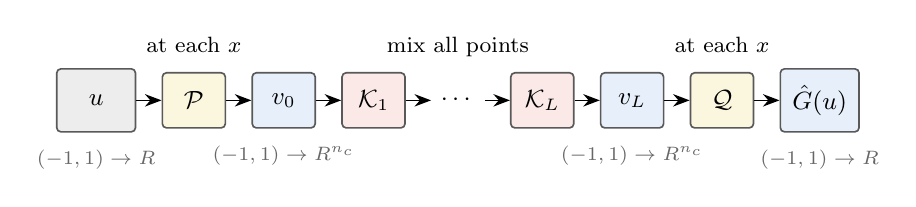
\begin{tikzpicture}[every node/.append style={font=\small}, node distance=4mm and 3.2mm,
    fn/.style={statenode, minimum width=8mm},
    pw/.style={opnode, minimum width=8mm, minimum height=7mm},
    mix/.style={layernode, fill=nodeGate, minimum width=8mm, minimum height=7mm},
    ch/.style={font=\scriptsize, text=black!60, below=1mm}]
  \node[inputnode, minimum width=10mm] (u) {$u$};
  \node[pw, right=of u]   (P)  {$\mathcal P$};
  \node[fn, right=of P]   (v0) {$\bm v_0$};
  \node[mix, right=of v0] (K1) {$\mathcal K_1$};
  \node[right=of K1]      (dd) {$\cdots$};
  \node[mix, right=of dd] (KL) {$\mathcal K_L$};
  \node[fn, right=of KL]  (vL) {$\bm v_L$};
  \node[pw, right=of vL]  (Q)  {$\mathcal Q$};
  \node[outputnode, right=of Q, minimum width=10mm] (out) {$\hat G(u)$};
  \foreach \a/\b in {u/P, P/v0, v0/K1, K1/dd, dd/KL, KL/vL, vL/Q, Q/out}
    \draw[edge] (\a) -- (\b);
  \node[ch] at (u.south)   {$(-1,1)\to\Real$};
  \node[ch] at (v0.south)  {$(-1,1)\to\Real^{n_c}$};
  \node[ch] at (vL.south)  {$(-1,1)\to\Real^{n_c}$};
  \node[ch] at (out.south) {$(-1,1)\to\Real$};
  % what each part does
  \node[font=\footnotesize, anchor=base] at ($(P.north)+(0,2.5mm)$) {at each $x$};
  \node[font=\footnotesize, anchor=base] at ($(Q.north)+(0,2.5mm)$) {at each $x$};
  \node[font=\footnotesize, anchor=base] at ($(K1.north)!0.5!(KL.north)+(0,2.5mm)$) {mix all points};
\end{tikzpicture}
\end{document}
